\documentclass[pdf,russian]{beamer}

\usepackage[T2A]{fontenc}
\usepackage[utf8]{inputenc}
\usepackage[russian]{babel}
\usepackage{booktabs}
\usepackage{minted}
\usepackage{tikz}
\usepackage{fancyvrb}
\usepackage{xcolor}
\usepackage{relsize}

\usetikzlibrary{trees}

\selectlanguage{russian}

\mode<presentation>{
    \usetheme{Frankfurt}
    \useoutertheme{infolines}
}

%% preamble
\title{Введение в git}
\author{Артем Оганджанян}
\institute{CSC}
\date{27 октября 2017 г.}

\begin{document}

\AtBeginSection[]
{
    \begin{frame}
        \frametitle{Оглавление}
        \tableofcontents
        [
            currentsection,
            subsectionstyle=show/show/hide
        ]
    \end{frame}
}

\begin{frame}
    \titlepage
\end{frame}

\section{Мотивация}

\subsection{История изменений}

\begin{frame}[fragile]
    \frametitle{Потеря кода}
    \pause
    Напишу-ка я тетрис.
    \begin{block}{}
        \begin{minted}{bash}
$ vim tetris.cpp
$ g++ tetris.cpp
$ ./a.out
        \end{minted}
    \end{block}
    \pause
    Добавлю разные уровни сложности...
    \begin{block}{}
        \begin{minted}{bash}
$ vim tetris.cpp
$ g++ tetris.cpp
$ ./a.out
        \end{minted}
    \end{block}
    \pause
    \only<+>{Работает!}
    \onslide<+->{Ой, что-то сломалось. Зря я код не сохранил\dots}
\end{frame}

\begin{frame}[fragile]
    \frametitle{Архивы}
    \begin{block}{}
        \begin{minted}{bash}
$ ls versions
        \end{minted}
        \texttt{\textcolor[HTML]{aa0000}{v0.1.tar}} \quad
        \texttt{\textcolor[HTML]{aa0000}{v0.2.tar}} \quad
        \pause
        \texttt{\textcolor[HTML]{aa0000}{v0.3.tar}} \quad
        \texttt{\textcolor[HTML]{aa0000}{v0.4.tar}} \quad
        \texttt{\textcolor[HTML]{aa0000}{v0.5.tar}} \quad
        \texttt{\textcolor[HTML]{aa0000}{v0.6.tar}} \quad
        \texttt{\textcolor[HTML]{aa0000}{v0.7.tar}} \quad
        \texttt{\textcolor[HTML]{aa0000}{v0.8.tar}} \quad
        \texttt{\textcolor[HTML]{aa0000}{v0.9.tar}}
    \end{block}
    \begin{itemize}
        \pause
        \item[$+$] Просто
        \pause
        \item[$-$] Неудобно
        \pause
        \item[$-$] Дублирование файлов
    \end{itemize}
\end{frame}

\subsection{Резервировное копирование}

\begin{frame}[fragile]
    \frametitle{Несчастные случаи}
    \begin{itemize}
        \pause
        \item Украли ноутбук
        \pause
        \item Утопили ноутбук
        \pause
        \item Умер жёсткий диск
    \end{itemize}
\end{frame}

\begin{frame}[fragile]
    \frametitle{Больше архивов}
    \begin{itemize}
        \item На флешке
        \item На Яндекс.Диске
    \end{itemize}
\end{frame}

\subsection{Командная работа}

\begin{frame}[fragile]
    \frametitle{Организация командной работы}
    Чат в телеграме:
    \begin{itemize}
        \pause
        \item[A:] Так, я сейчас сделаю это.
        \pause
        \item[B:] А я это сделаю.
        \pause
        \item[C:] Ой, тут баг есть, сейчас поправлю.
        \pause
        \item[A:] Стой! Не трогай тот код, я его сейчас изменяю.
        \pause
        \item[D:] Привет, я вернулся. У кого сейчас последняя версия исходников?
        \pause
        \item[B:] Я закончил.
        \pause
        \item[A:] Блин, я тоже тот файл правил...
    \end{itemize}
\end{frame}

\begin{frame}[fragile]
    \frametitle{Организация командной работы}
    Больше людей "--- ещё хуже.
    \pause
    Как решать проблему?
\end{frame}

\section{Принцип работы}

\subsection{Структура}

\begin{frame}[fragile]
    \frametitle{Структура хранилища}

    \only<3-4>{Список версий?}
    \only<5-6>{Дерево версий?}
    \onslide<7->{Ациклический граф версий\onslide<8->{, указатели}}

    \newcommand{\sinceOne}[1]{\onslide<2->{#1}}
    \newcommand{\sinceTwo}[1]{\onslide<4->{#1}}
    \newcommand{\sinceThree}[1]{\onslide<6->{#1}}
    \newcommand{\sinceFour}[1]{\onslide<8->{#1}}

    \begin{block}{}
        \begin{Verbatim}[commandchars=\\\{\}]
\sinceThree{* \textcolor[HTML]{aa5500}{995aadd}\sinceFour{\textcolor[HTML]{aa5500}{ (}\textcolor[HTML]{00aaaa}{HEAD}\textcolor[HTML]{aa5500}{ -> }\textcolor[HTML]{00aa00}{dev}\textcolor[HTML]{aa5500}{)}} Add main.cpp}
\sinceThree{*   \textcolor[HTML]{aa5500}{72a5b82}\sinceFour{\textcolor[HTML]{aa5500}{ (}\textcolor[HTML]{aa0000}{origin/dev}\textcolor[HTML]{aa5500}{)}} Merge branch 'manual'}
\sinceThree{\textcolor[HTML]{00aa00}{|}\textcolor[HTML]{aa5500}{\textbackslash}}
\sinceThree{\textcolor[HTML]{00aa00}{|}} \sinceTwo{* \textcolor[HTML]{aa5500}{514cae7}\sinceFour{\textcolor[HTML]{aa5500}{ (}\textcolor[HTML]{aa0000}{origin/manual}\textcolor[HTML]{aa5500}{, }\textcolor[HTML]{00aa00}{manual}\textcolor[HTML]{aa5500}{)}} Finish working on man}
\sinceThree{\textcolor[HTML]{00aa00}{|}} \sinceTwo{* \textcolor[HTML]{aa5500}{f44e819} Start working on man}
\sinceOne{*} \sinceTwo{\textcolor[HTML]{aa5500}{|}} \sinceOne{\textcolor[HTML]{aa5500}{ea84576} Update README.md}
\sinceOne{\textcolor[HTML]{aa5500}{|}}\sinceTwo{\textcolor[HTML]{aa5500}{/}}
\sinceOne{* \textcolor[HTML]{aa5500}{eefea48} Add LICENCE}
\sinceOne{* \textcolor[HTML]{aa5500}{53f3d7a} Add README.md}
        \end{Verbatim}
    \end{block}
\end{frame}

\begin{frame}
    \frametitle{Buzzwords}
    \begin{itemize}
        \pause
        \item Система контроля версий, version control system, VSC.
        \pause
        \item Репозиторий.
        \pause
        \item Версия "--- commit.
        \pause
        \item Указатель "--- branch. \pause Не обязательно выглядит как ветка.
    \end{itemize}
\end{frame}

\begin{frame}
    \frametitle{Копии файлов}
    \begin{itemize}
        \pause
        \item На каждый commit создаётся копия всех изменённых файлов.
        \pause
        \item Файлы, которые не менялись, не копируются.
        \pause
        \item Можно было бы хранить только изменения (diff) файлов.
            \pause Но git этого не делает.
        \pause
        \item Зато git (по умолчанию) сжимает файлы.
    \end{itemize}
\end{frame}

\subsection{Децентрализация}

\begin{frame}
    \frametitle{git "--- децентрализованная VCS}
    \begin{figure}
        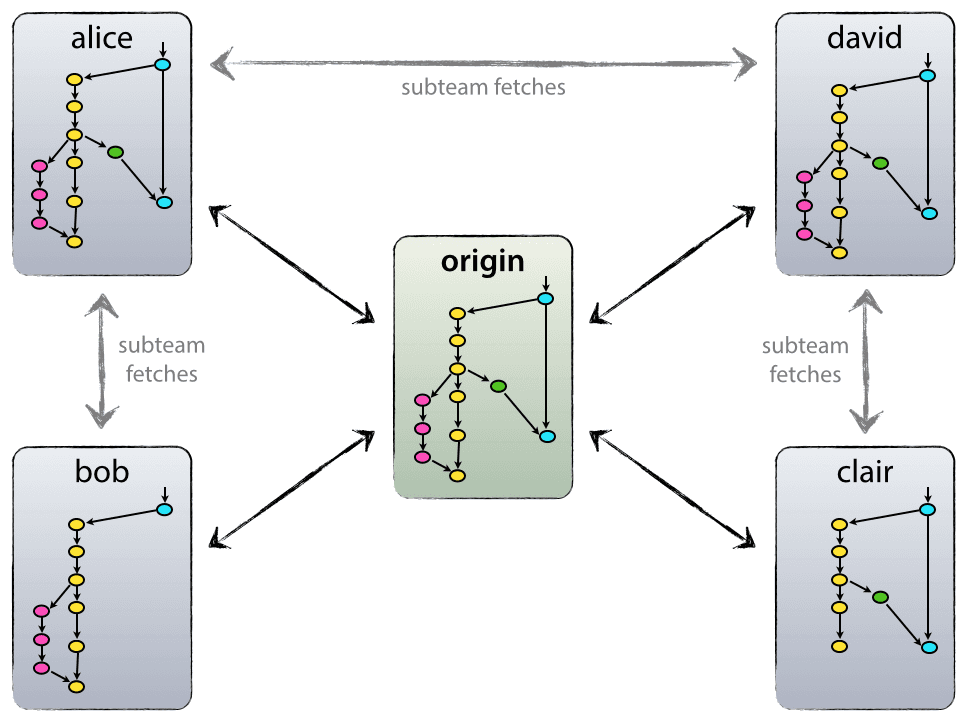
\includegraphics[height=0.8\textheight]{decentr}
    \end{figure}
\end{frame}

\begin{frame}
    \frametitle{Преимущества}
    \begin{itemize}
        \pause
        \item Локальные изменения
        \pause
        \item Отказоустойчивость
        \pause
        \item Довольный Линус
    \end{itemize}
\end{frame}

\begin{frame}
    \frametitle{Довольный Линус}
    \begin{figure}
        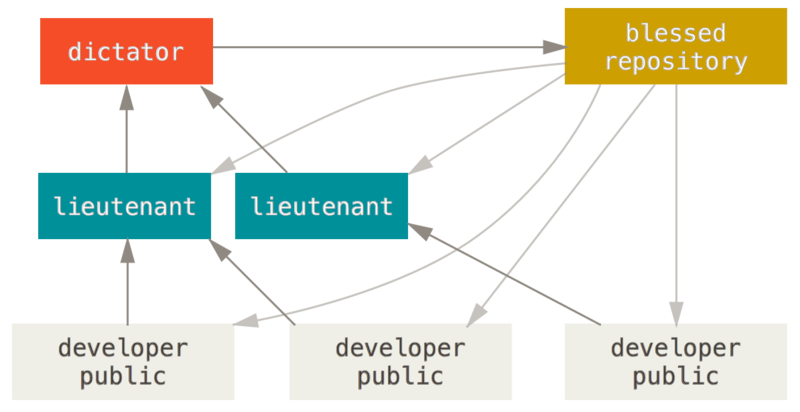
\includegraphics[width=\textwidth]{dictator}
    \end{figure}
\end{frame}

\section{Основные команды}

\begin{frame}[fragile]
    \frametitle{Самый бесполезный раздел}
    \pause
    \center
    \only<+>{
\includegraphics[height=0.8\textheight,keepaspectratio]{alice.jpg}}
    \onslide<+->
    \begin{Verbatim}[fontsize=\relsize{-3}]
$ git
usage: git [--version] [--help] [-C <path>] [-c name=value]
           [--exec-path[=<path>]] [--html-path] [--man-path] [--info-path]
           [-p | --paginate | --no-pager] [--no-replace-objects] [--bare]
           [--git-dir=<path>] [--work-tree=<path>] [--namespace=<name>]
           <command> [<args>]

These are common Git commands used in various situations:

start a working area (see also: git help tutorial)
   clone      Clone a repository into a new directory
   init       Create an empty Git repository or reinitialize an existing one

work on the current change (see also: git help everyday)
   add        Add file contents to the index
   mv         Move or rename a file, a directory, or a symlink
   reset      Reset current HEAD to the specified state
   rm         Remove files from the working tree and from the index

examine the history and state (see also: git help revisions)
   bisect     Use binary search to find the commit that introduced a bug
   grep       Print lines matching a pattern
   log        Show commit logs
   show       Show various types of objects
   status     Show the working tree status
    \end{Verbatim}
\end{frame}

\subsection{Начало работы}

\begin{frame}
    \frametitle{Установка}
    \onslide<1->\mintinline{bash}{$ sudo apt install git} \\
    \onslide<1->\mintinline{bash}{$ git config}
    \onslide<3->\mintinline{bash}{ --help}\\
    \onslide<4->\mintinline{bash}{$ man git-config}
    \onslide<2->
    \begin{exampleblock}{Пример}
        \mintinline{bash}{$ git config --global user.name "Artem Ohanjanyan"}
        \mintinline{bash}{$ git config --global user.email artemohanjanyan@gmail.com}
        \mintinline{bash}{$ git config --global core.editor vim}
    \end{exampleblock}
\end{frame}

\begin{frame}
    \frametitle{Получение репозитория}
    \begin{itemize}
        \item<2-> \mintinline{bash}{$ git init}
            \onslide<5->{\mintinline{bash}{ --help}}
        \item<3-> \mintinline{bash}{$ git clone}
            \onslide<5->{\mintinline{bash}{ --help}}
    \end{itemize}
    \onslide<4->
    \begin{exampleblock}{Пример}
        \mintinline{bash}{git clone https://github.com/artemohanjanyan/git-tutorial.git}
    \end{exampleblock}
\end{frame}

\subsection{Учёт изменений}

\begin{frame}
    \frametitle{Жизненный цикл файла}
    \center
    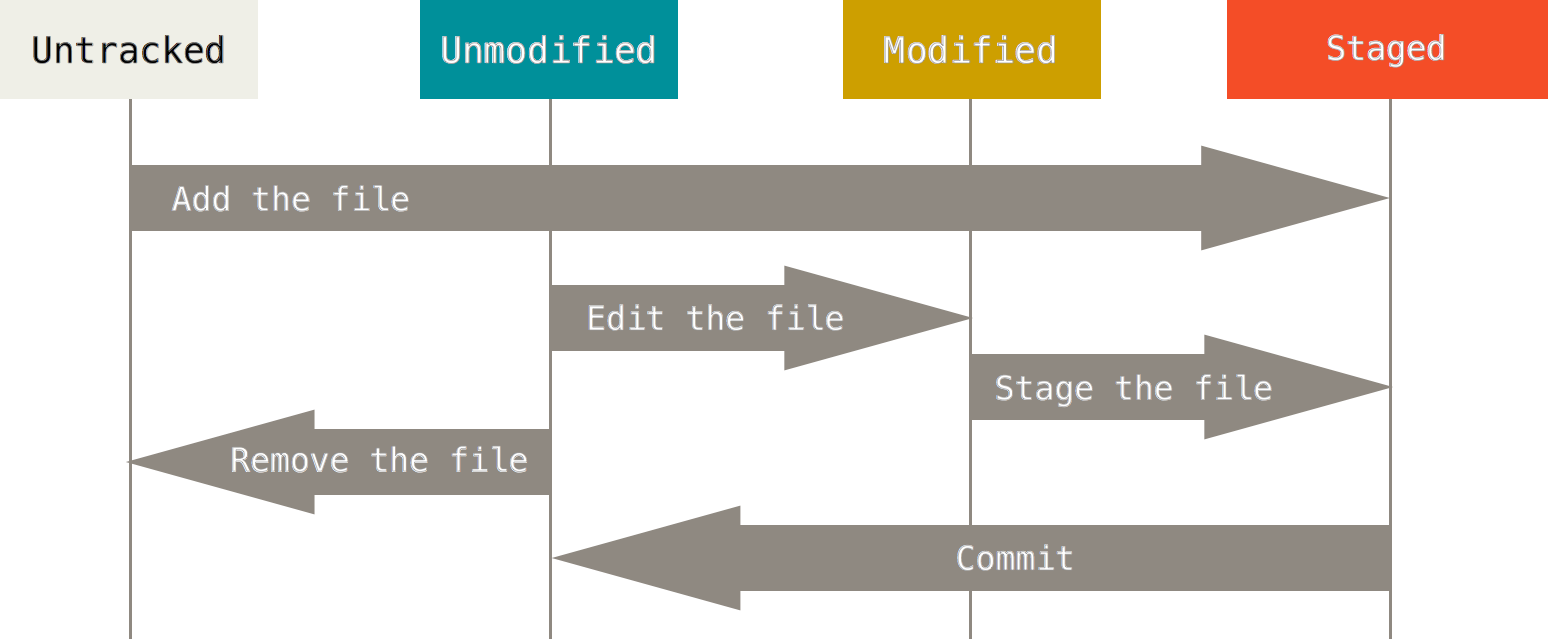
\includegraphics[width=0.9\textwidth]{lifecycle}
\end{frame}

\begin{frame}
    \frametitle{Команды}
    \begin{itemize}
        \item<1-> \mintinline{bash}{$ git add}
            \onslide<3->{\mintinline{bash}{ --help}}
        \item<1-> \mintinline{bash}{$ git mv}
            \onslide<3->{\mintinline{bash}{ --help}}
        \item<1-> \mintinline{bash}{$ git reset}
            \onslide<3->{\mintinline{bash}{ --help}}
        \item<1-> \mintinline{bash}{$ git rm}
            \onslide<3->{\mintinline{bash}{ --help}}
    \end{itemize}
    \onslide<2->
    \begin{exampleblock}{Пример}
        \mintinline{bash}{$ git add slides.tex}\\
        \mintinline{bash}{$ git mv dictator.png img/}
    \end{exampleblock}
\end{frame}

\subsection{Проверка}

\begin{frame}[fragile]
    \frametitle{Команды}
    \begin{itemize}
        \item<1-> \mintinline{bash}{$ git status}
            \onslide<3->{\mintinline{bash}{ --help}}
        \item<1-> \mintinline{bash}{$ git log}
            \onslide<3->{\mintinline{bash}{ --help}}
    \end{itemize}
    \onslide<2->
    \begin{exampleblock}{Пример}
        \begin{Verbatim}[fontsize=\relsize{-3},commandchars=\\\{\}]
On branch master
Your branch is up-to-date with 'origin/master'.
Changes to be committed:
  (use "git reset HEAD <file>..." to unstage)

	\textcolor[HTML]{00aa00}{modified:   Makefile}

Changes not staged for commit:
  (use "git add <file>..." to update what will be committed)
  (use "git checkout -- <file>..." to discard changes in working directory)

	\textcolor[HTML]{aa0000}{modified:   slides.tex}

Untracked files:
  (use "git add <file>..." to include in what will be committed)

	\textcolor[HTML]{aa0000}{alice.jpg}
	\textcolor[HTML]{aa0000}{lifecycle.png}
        \end{Verbatim}
    \end{exampleblock}
\end{frame}

\begin{frame}[fragile]
    \frametitle{Команды}
    \begin{exampleblock}{Пример}
        \begin{Verbatim}[commandchars=\\\{\}]
$ git log --graph --decorate --oneline
* \textcolor[HTML]{aa5500}{995aadd}\textcolor[HTML]{aa5500}{ (}\textcolor[HTML]{00aaaa}{HEAD}\textcolor[HTML]{aa5500}{ -> }\textcolor[HTML]{00aa00}{dev}\textcolor[HTML]{aa5500}{)} Add main.cpp
*   \textcolor[HTML]{aa5500}{72a5b82}\textcolor[HTML]{aa5500}{ (}\textcolor[HTML]{aa0000}{origin/dev}\textcolor[HTML]{aa5500}{)} Merge branch 'manual'
\textcolor[HTML]{00aa00}{|}\textcolor[HTML]{aa5500}{\textbackslash}
\textcolor[HTML]{00aa00}{|} * \textcolor[HTML]{aa5500}{514cae7}\textcolor[HTML]{aa5500}{ (}\textcolor[HTML]{aa0000}{origin/manual}\textcolor[HTML]{aa5500}{, }\textcolor[HTML]{00aa00}{manual}\textcolor[HTML]{aa5500}{)} Finish working on man
\textcolor[HTML]{00aa00}{|} * \textcolor[HTML]{aa5500}{f44e819} Start working on man
* \textcolor[HTML]{aa5500}{|} \textcolor[HTML]{aa5500}{ea84576} Update README.md
\textcolor[HTML]{aa5500}{|}\textcolor[HTML]{aa5500}{/}
* \textcolor[HTML]{aa5500}{eefea48} Add LICENCE
* \textcolor[HTML]{aa5500}{53f3d7a} Add README.md
        \end{Verbatim}
    \end{exampleblock}
\end{frame}

\subsection{Внесение изменений}
\begin{frame}
    \frametitle{Команды}
    \begin{itemize}
        \item<1-> \mintinline{bash}{$ git commit}
            \onslide<7->{\mintinline{bash}{ --help}}
        \item<2-> \mintinline{bash}{$ git checkout}
            \onslide<7->{\mintinline{bash}{ --help}}
        \item<3-> \mintinline{bash}{$ git diff}
            \onslide<7->{\mintinline{bash}{ --help}}
        \item<4-> \mintinline{bash}{$ git merge}
            \onslide<7->{\mintinline{bash}{ --help}}
        \item<5-> \mintinline{bash}{$ git branch}
            \onslide<7->{\mintinline{bash}{ --help}}
        \item<6-> \mintinline{bash}{$ git tag}
            \onslide<7->{\mintinline{bash}{ --help}}
    \end{itemize}
\end{frame}

\begin{frame}
    \frametitle{git commit}
    \center
    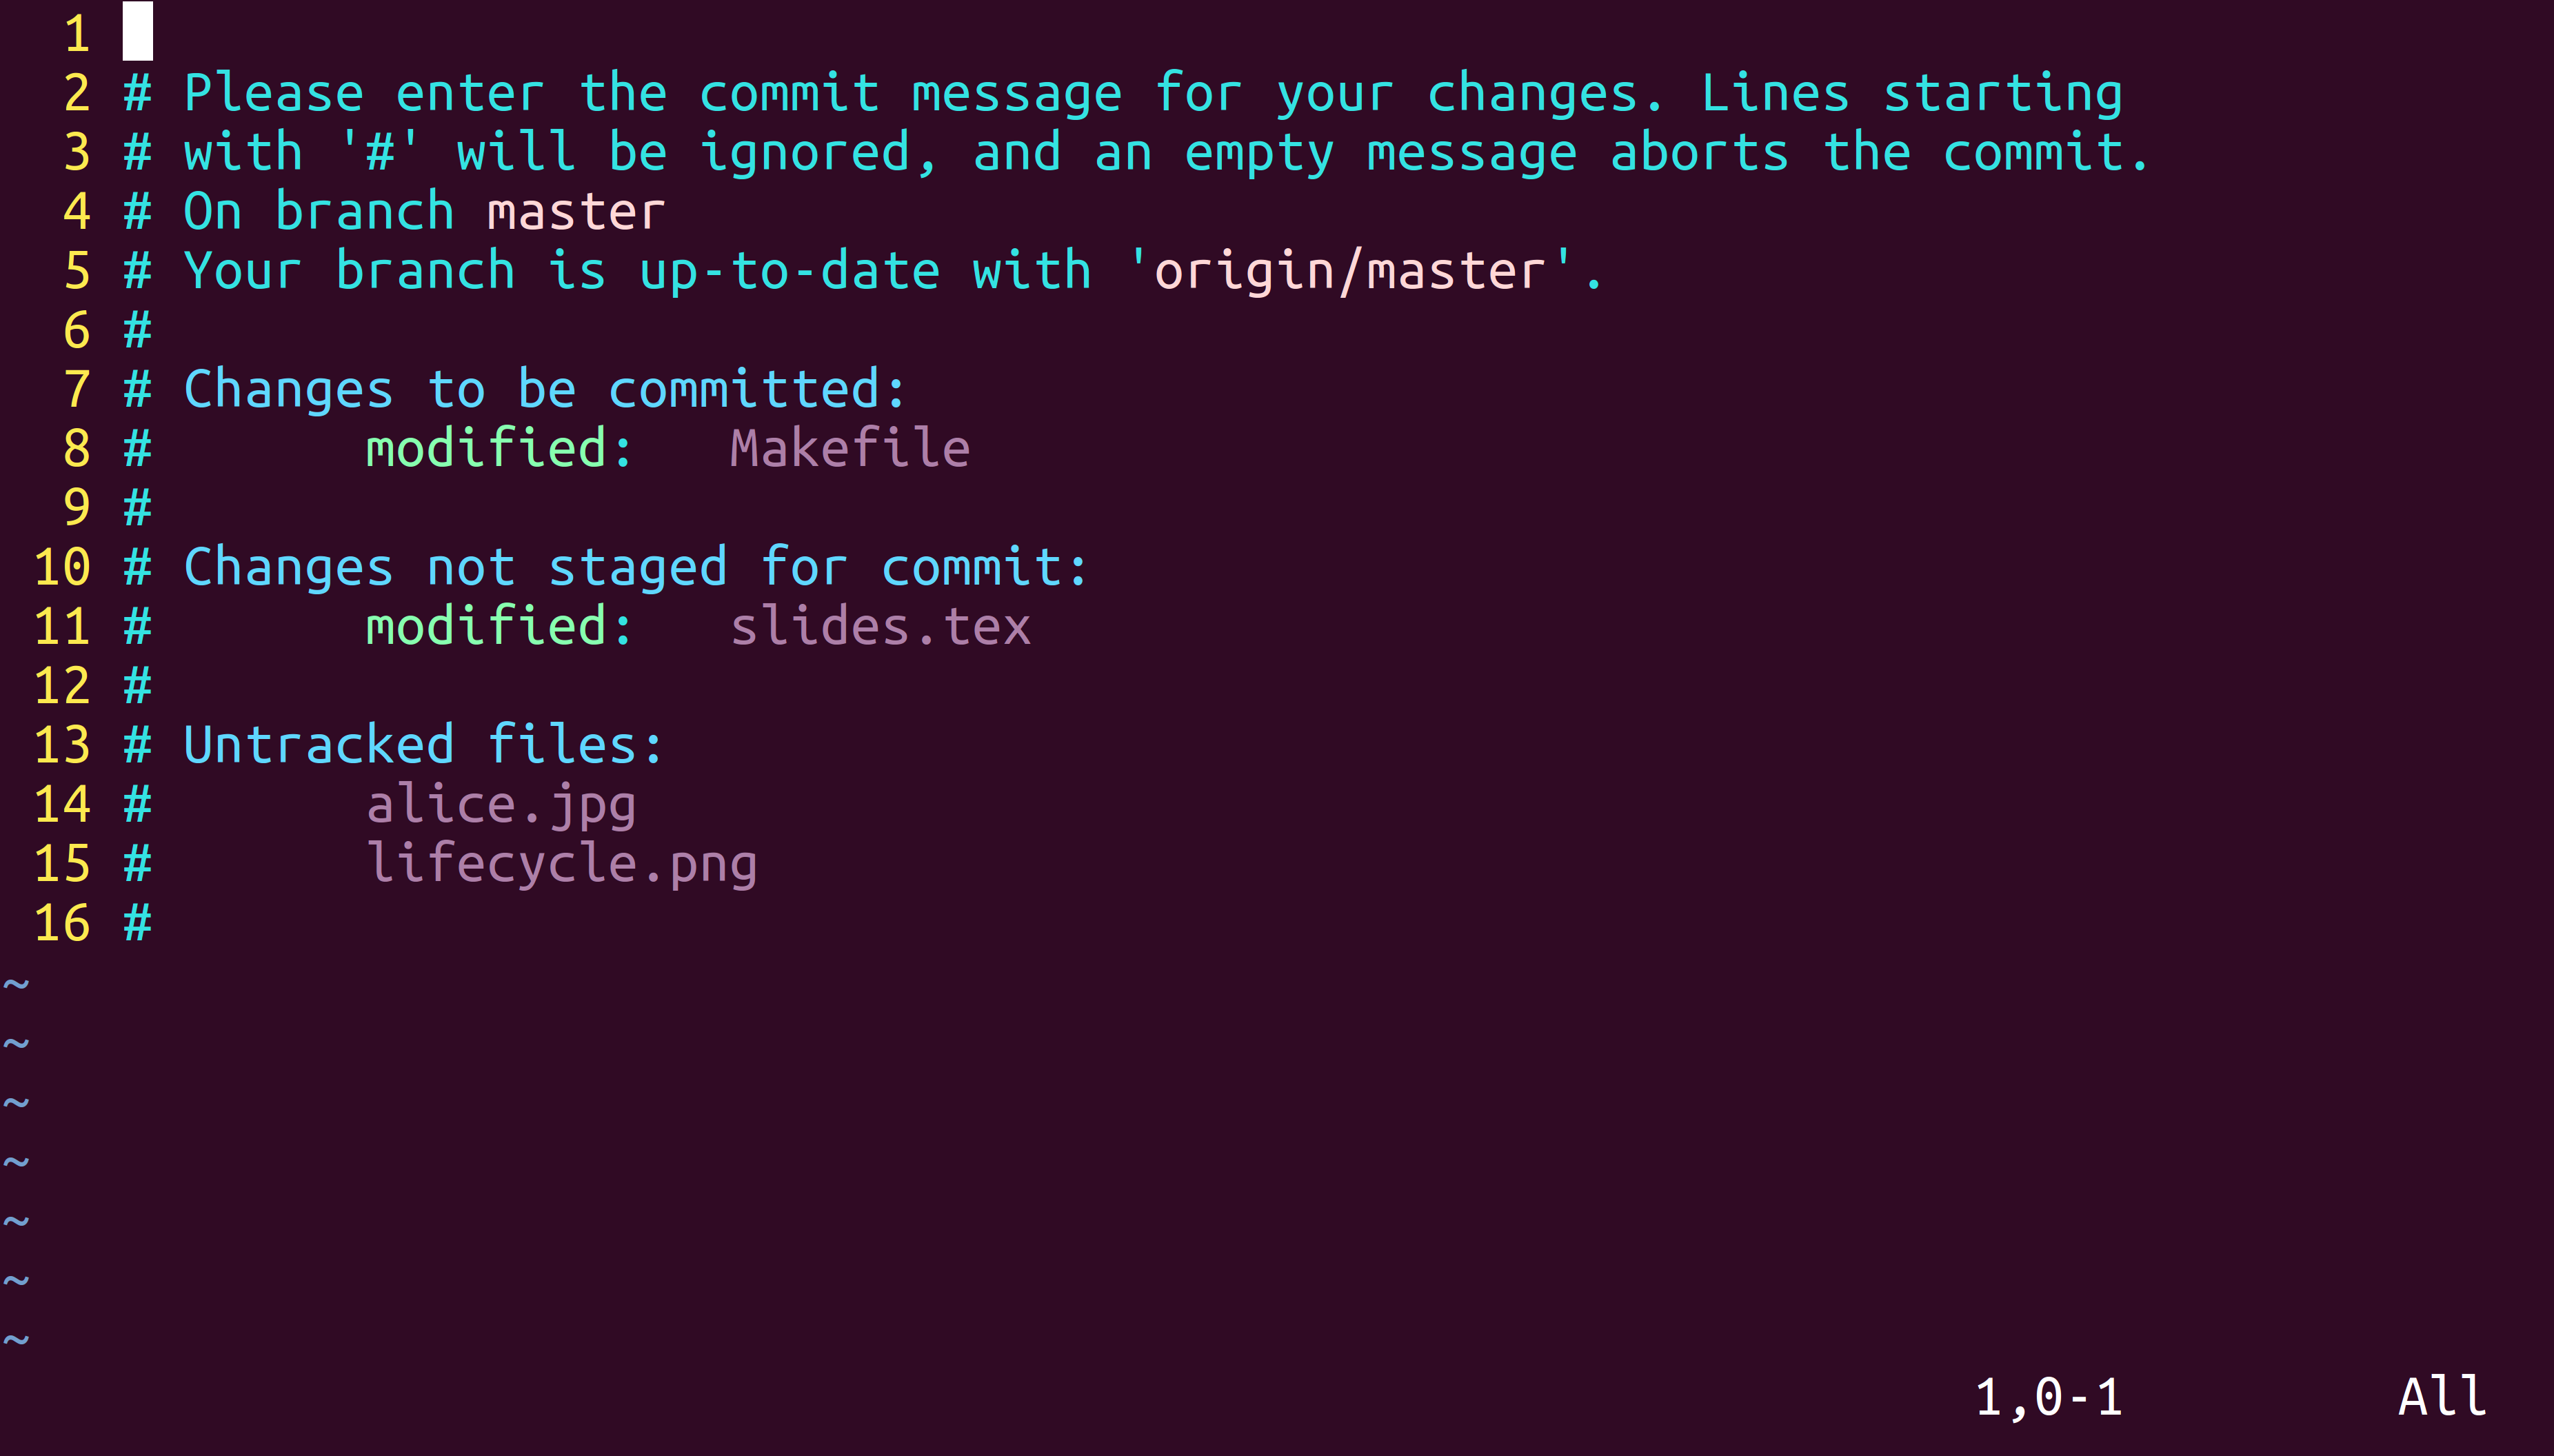
\includegraphics[width=0.95\textwidth]{vim}
\end{frame}

\begin{frame}
    \frametitle{git checkout}
    \center
    \begin{itemize}
        \pause
        \item \mintinline{bash}{$ git checkout master}
        \pause
        \item \mintinline{bash}{$ git checkout 6be2821}
        \pause
        \item \mintinline{bash}{$ git checkout -b feature}
    \end{itemize}
\end{frame}

\begin{frame}[fragile]
    \frametitle{git merge}
    \begin{itemize}
        \pause
        \item \mintinline{bash}{$ git merge feature}
        \pause
        \item merge-конфликты
    \end{itemize}
    \pause
    \begin{exampleblock}{Пример}
        \begin{Verbatim}
<<<<<<< HEAD
Changes on master
=======
Changes on feature
>>>>>>> feature
        \end{Verbatim}
    \end{exampleblock}
\end{frame}

\begin{frame}
    \frametitle{Ссылки на коммиты}
    \begin{itemize}
        \pause
        \item \texttt{HEAD}, \texttt{master}
        \pause
        \item \texttt{HEAD\~{}}
        \pause
        \item \texttt{HEAD\~{}\~{}\~{}}
        \pause
        \item \texttt{HEAD\~{}10}
        \pause
        \item \texttt{HEAD\^{}\^{}}
        \pause
        \item \mintinline{bash}{$ man git-rev-parse}
    \end{itemize}
\end{frame}

\begin{frame}[fragile]
    \begin{minted}{bash}
$ history | grep -P "^(\s|\d)*git" | awk '{ print $2, $3 }'
          | sort | uniq -c | sort -n -r | head -n 13
    304 git add
    300 git commit
    244 git checkout
    148 git push
    131 git diff
    110 git clone
     75 git rm
     69 git merge
     68 git remote
     62 git branch
     47 git reset
     45 git mv
     25 git log
     17 git pull
     14 git check-ignore
    \end{minted}
\end{frame}

\section{Советы}

\section{Продвинутые команды}

\section{GitHub}

\end{document}
